%%%%%%%%%%%%%%%%%%%%%%%%%%%%%%%%%%%%%%%%%%%%%%%%%%%%%%%%%%%%%%%%%%%%%%%%%
% This file is part of the LaTeX sources of the OMDoc 1.3 specification
% Copyright (c) 2006 Michael Kohlhase
% This work is licensed by the Creative Commons Share-Alike license
% see http://creativecommons.org/licenses/by-sa/2.5/ for details
%%%%%%%%%%%%%%%%%%%%%%%%%%%%%%%%%%%%%%%%%%%%%%%%%%%%%%%%%%%%%%%%%%%%%%%%%

\begin{tchapter}[id=omdoc-markup,short=Open Mathematical Documents]{OMDoc: Open Mathematical Documents}

  Based on the analysis of the structure inherent in mathematical knowledge and existing
  content markup systems for mathematics we will now briefly introduce basic design
  assumptions and the development history of the {\omdoc} format, situate it, and discuss
  possible applications.

  \begin{tsection}[id=omdoc-history]{A Brief History of the {\omdoc} Format}
    {\omdoc} initially developed from the quest for a solution of the problem of
    representing knowledge on the one hand and integrating external mathematical reasoning
    systems in the {\OMEGA} project at Saarland University on the
    other. {\OMEGA}~\cite{SiekmannEtAl:pdwo02} is a large-scale
    {\atwintoo{proof}{development}{environment}} that integrates various reasoning engines
    ({\atwintoo{automated}{theorem}{prover}s}, {\twintoo{decision}{procedure}s},
    {\twintoo{computer algebra}{system}s}) via
    {\atwintoo{knowledge-based}{proof}{planning}} with the aim of creating a
    {\atwintoo{mathematical}{assistant}{system}}.

    \begin{tsubsection}{The Design Problem}
      One of the hard practical problems of building such systems is to represent,
      provision, and manage the relevant (factual\twin{factual}{knowledge}, tactic, and
      intuitive\twin{intuitive}{knowledge}) knowledge human mathematicians use in
      developing mathematical theories and proofs: Knowledge-based reasoning systems use
      explicit representations of this knowledge to automate the search for a proof, and
      before a system can be applied to a mathematical domain it must be formalized, the
      proof tactics of this domain must be identified, and the intuitions of when to use
      which tactic must be coaxed from practitioners. Ideally, as a valuable and expensive
      resource, this knowledge would be shared between mathematical assistant systems to
      be able to compare the relative strength of the systems and to enhance practical
      coverage. This poses the problem that the knowledge must be represented at a level
      that would accommodate the different systems' representational quirks and bridge
      between them.

      Developing an agent-oriented framework for distributed reasoning via remote
      procedure calls to achieve system scalability
      (\mathwebsb~\cite{FraKoh:mabdl99,ZimKoh:tmsbdmr02}; see {\mychapref{rpc}} for an
      {\omdoc}-based reformulation) revealed that the underlying problem in integrating
      mathematical systems is a semantic one: all the reasoning systems make differing
      ontological assumptions that have to be reconciled to achieve a correct
      (i.e. meaning-preserving) integration. This integration problem is quite similar to
      the one at the knowledge level: if the knowledge ingrained in the system design
      could be explicitly described, then it would be possible to find applicable systems
      and deploy the necessary (syntactic) and (semantic) bridges automatically.

      The approaches and solutions offered by the automated reasoning communities at that
      time were insular at best: They standardized character-level syntax standardizing on
      first-order logic~\cite{SuSu94,HaeKerWei:csdfgsd96}, or explored bilateral system
      integrations overcoming deep ontological discrepancies between the
      systems~\cite{FelHow:hitpnh97}.

      At the same time, (ca 1998) the Computer Algebra Community was grappling with
      similar integration problems. The {\openmath} standard that was emerging shad solved
      the web-scalability problem in representing mathematical formulae by adopting the
      emerging {\xml} framework as a syntactical basis and providing structural markup
      with explicit context references as a syntax-independent representation
      approach. First attempts by the author to influence {\openmath} standardization so
      that the format would allow mathematical knowledge representation (i.e. the
      statements and context level) were unsuccessful. The {\openmath} community had
      intensively discussed similar issues under the heading of ``content dictionary
      inheritance'' and ``conformance specification'', and had decided that they were too
      controversial for standardization.
  \end{tsubsection}

  \begin{tsubsection}{Design Principles}
    The start of the development of {\omdoc} as a content-based representation format for
    mathematical knowledge was triggered by an e-mail by {\twintoo{Alan}{Bundy}} to the
    author in 1998, where he lamented the fact that one of the great hindrances of
    knowledge-based reasoning is the fact that formalizing mathematical knowledge is very
    time-consuming and that it is very hard for young researchers to gain recognition for
    formalization work. This led to the idea of developing a global repository of
    formalized mathematics, which would eventually allow peer-reviewed publication of
    formalized mathematical knowledge, thus generating academic recognition for
    formalization work and eventually lead to the much enlarged corpus of formalized
    mathematics that is necessary for knowledge-based formal mathematical reasoning. Young
    researchers would contribute formalizations of mathematical knowledge in the form of
    mathematical documents that would be both formal and thus machine-readable, as well as
    human-readable, so that humans could find and understand them\footnote{Here the strong
      influence of the {\mizar} project under {\twintoo{Andrzej}{Trybulec}} must be
      acknowledged, at that time, the project had already realized these two goals. They
      had even established the ``Journal of Formalized Mathematics'', where {\LaTeX}
      articles were generated from the automatically verified {\mizar} source. However,
      the {\mizar} mathematical language~\cite{URL:MizarLanguage} used a human-oriented
      syntax that defied outside parsing and web-integration, had a tightly integrated
      largely undocumented sort system, and made very strong ontological commitments.}.
      
    This idea brought the final ingredient to the design principles: in a nutshell, the
    {\omdoc} format was to 
    \begin{enumerate}
    \item\label{item:ontological-flexibility} be {\emph{Ontologically uncommitted}} (like
      the {\openmath} format), so that it could serve as a {\emph{integration format}} for
      mathematical software systems.
    \item\label{item:documents} provide a representation format for {\emph{mathematical
          documents}} that combined {\emph{formal}} and {\emph{informal}} views of all the
      {\emph{mathematical knowledge}} contained in them.
    \item\label{item:logic} be based on {\emph{sound logic/representational principles}}
      (as not to embarrass the author in front of his colleagues from automated reasoning)
    \item\label{item:content-markup} be based on {\emph{structural/content markup}} to
      guarantee both~\ref{item:ontological-flexibility}.) and~\ref{item:documents}.).
    \end{enumerate}
  \end{tsubsection}
  
  \begin{tsubsection}{Development History} 
    Version 1.0 of the {\omdoc} format was released on November $1^{st}$ 2000 to give
    users a stable interface to base their documents and systems on. It was adopted by
    various projects in {\twintoo{automated}{deduction}},
    {\twintoo{algebraic}{specification}}, and
    {\twintoo{computer-supported}{education}}. The experience from these projects
    uncovered a multitude of small deficiencies and extension possibilities of the format,
    that have been subsequently discussed in the {\omdoc} {\indextoo{community}}.

    {\omdocv{1.1}} was released on December $29^{th}$ 2001 as an attempt to roll the
    uncontroversial and non-disruptive part of the extensions and corrections into a
    consistent language format. The changes to version 1.0 were largely conservative,
    adding optional attributes or child elements. Nevertheless, some non-conservative
    changes were introduced, but only to less used parts of the format or in order to
    remedy design flaws and inconsistencies of version 1.0.

\begin{oldpart}{adapt}
    {\omdocv{1.2}} is the mature version in the {\omdocv{1}} series of specifications. It
    contains almost no large-scale changes to the document format, except that {\cmathml}
    is now allowed as a representation for mathematical objects. But many of the
    representational features have been fine-tuned and brought up to date with the
    maturing {\xml} technology (e.g. {\snippet{ID}}\twin{type}{ID} attributes now follow
    the XML ID specification~\cite{XML:id05}, and the Dublin Core elements follow the
    official syntax~\cite{DCMI:dmt03}). The main development is that the {\omdoc}
    specification, the DTD, and schema are split into a system of interdependent modules
    that support independent development of certain language aspects and simpler
    specification and deployment of sub-languages.  {\vomdoc{1.2}} freezes the development
    so that version 2 can be started off on the modules.
  \end{oldpart}
\end{tsubsection}
\end{tsection}

\begin{tsection}[id=three-level-markup]{Three Levels of Markup}

  To achieve content\twin{content}{markup} and {\twintoo{context}{markup}} for
  mathematical knowledge, {\omdoc} uses three levels of modeling corresponding to the
  concerns raised previously. We have visualized this architecture in
  {\myfigref{nutshell}}.

\begin{myfig}{nutshell}{{\omdoc} in a Nutshell (the Three Levels of Modeling)}
\renewcommand{\arraystretch}{.2}
\begin{tabular}{|p{5.2cm}|p{5.4cm}|}\hline
   Level  of Representation & {\omdoc} Example\\\hline\hline
{\emph{Theory Level}:} Development Graph
    \begin{itemize}
    \item Inheritance via symbol-mapping
    \item Theory inclusion via proof-obligations
    \item Local (one-step)\twin{local}{link} vs. {\twintoo{global}{link}s}
    \end{itemize}&
    \begin{minipage}{5.3cm}\vspace*{1ex}\tiny
      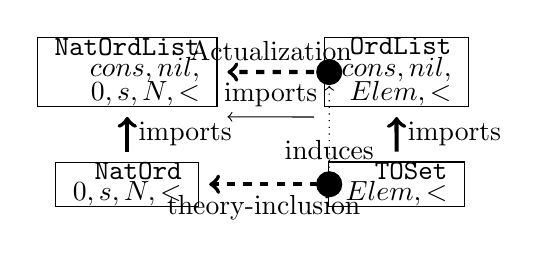
\begin{tikzpicture}[scale=.57]  \node (natordlist) at (0,2.5) 
    {\begin{tabular}{|r|}\hline 
      {\tt{NatOrdList}}\\
      $cons, nil,$\\
      $0,s,{\mathbb{N}},<$\\\hline
    \end{tabular}};
  \node (natord) at (0,0) 
    {\begin{tabular}{|r|}\hline 
      {\tt{NatOrd}}\\
      $0,s,{\mathbb{N}},<$\\\hline
    \end{tabular}};
  \node (toset) at (6,0) 
    {\begin{tabular}{|r|}\hline 
      {\tt{TOSet}}\\
      $Elem,<$\\\hline
    \end{tabular}};
  \node (ordlist) at (6,2.5) 
    {\begin{tabular}{|r|}\hline 
      {\tt{OrdList}}\\
      $cons, nil,$\\
      $Elem,<$\\\hline
    \end{tabular}};
  \node[circle,fill] (act1) at (4.5,2.5) {};
  \node[circle,fill] (act2) at (4.5,0) {};
  \draw [->,line width=1.5pt] (natord) -- node[right]{imports} (natordlist);
  \draw [->,line width=1.5pt] (toset) -- node[right]{imports} (ordlist);
  \draw [->,dashed,line width=1.5pt] (toset) -- node[below]{theory-inclusion} (natord);
  \draw [->,dashed,line width=1.5pt] (ordlist) -- node[above]{Actualization} (natordlist);
  \draw [->] (ordlist.south west) -- node[above]{imports} (natordlist.south east);
  \draw [<-,dotted,near end] (act1) -- node{induces} (act2);
\end{tikzpicture}
      \vspace*{-1.6cm}
    \end{minipage}\\[-1ex]\hline
 {\emph{Statement Level}:} 
    \begin{itemize}
    \item Axiom, definition, theorem, proof, example,\ldots
    \item Structure explicit in statement forms and references
    \end{itemize}&
{\footnotesize\baselineskip=10pt\strut\vspace*{-3ex}
\begin{lstlisting}[numbers=none,frame=none,mathescape]
<definition for="plus" type="recursive">
 <CMP><xhtml:p>Addition is defined by
   recursion on the second argument.</xhtml:p>
 </CMP>
 <FMP>$X+0=0$</FMP> 
 <FMP>$X+s(Y)=s(X+Y)$</FMP> 
</definition>
\end{lstlisting}}\\[-3ex]\hline
   {\emph{Object Level}:} {\openmath}/{\mathml}
    \begin{itemize}
    \item Objects as logical formulae
    \item Semantics by pointing to theory level
    \end{itemize} &
{\begin{minipage}[t]{5.4cm}\footnotesize\baselineskip=10pt\strut\vspace*{-3ex}
\begin{lstlisting}[numbers=none,frame=none]
<OMA>
 <OMS cd="arith1" name="plus"/>
 <OMV name="X"/>
 <OMS cd="nat" name="zero"/>
</OMA>
\end{lstlisting}\vspace{-3ex}\end{minipage}}\\\hline
\end{tabular}
\end{myfig}
Building on the discussion in {\mychapref{math-markup}} we distinguish three levels of
representation in {\omdoc}
\begin{description}
\item[\emph{Mathematical Theories} (see {\mysecref{math-objects}})] At this level,
  {\omdoc} supplies original markup for clustering sets of statements into theories, and
  for specifying relations between theories by morphisms. By using this scheme,
  mathematical knowledge can be structured into reusable chunks. Theories also serve as
  the primary notion of context in {\omdoc}, they are the natural target for the context
  aspect of formula and statement markup.
\item[\emph{Mathematical Statements} (see {\mysecref{meta-math}})] {\omdoc} provides
  original mark\-up infrastructure for making the structure of mathematical statements
  explicit.  Again, we have content and context markup aspects. For instance the
  definition in the right hand side of the second row of {\myfigref{nutshell}} contains an
  informal description of the definition as a first child and a formal description in the
  two recursive equations in the second and third children supported by the
  {\attribute{type}{definition}} attribute, which states that this is a recursive
  definition. The context markup in this example is simple: it states that this piece of
  markup pertains to a symbol declaration for the symbol {\snippetin{plus}} in the current
  theory (presumably the theory {\snippetin{arith1}}).
\item[\emph{Mathematical Formulae} (see {\mysecref{meta-theories}})] At the level of
  mathematical formulae, {\omdoc} uses the established standards
  {\openmath}~\cite{BusCapCar:2oms04} and {\cmathml}~\cite{CarIon:MathML03}.  These
  provide content markup for the structure of mathematical formulae and context markup in
  the form of URI references in the symbol representations (see {\mychapref{mobj}} for an
  introduction).
\end{description}
All levels are augmented by markup for various auxiliary information that is
present in mathematical documents, e.g. notation declarations, exercises,
experimental data, program code, etc.
\end{tsection}

\begin{tsection}[id=situating]{Situating the OMDoc Format}

  The space of representation languages for mathematical knowledge reaches from the input
  languages of {\twintoo{computer algebra}{system}s}\twin{algebra}{system} (CAS) to
  presentation markup languages for mathematical vernacular like {\TeX/\LaTeX}. We have
  organized some of the paradigmatic examples in a diagram mapping coverage (which kinds
  of mathematical knowledge can be expressed) against machine support (which services the
  respective software system can offer) in {\myfigref{situating}}.

\begin{myfig}{situating}{Situating Content Markup: Math. Knowledge Management}
  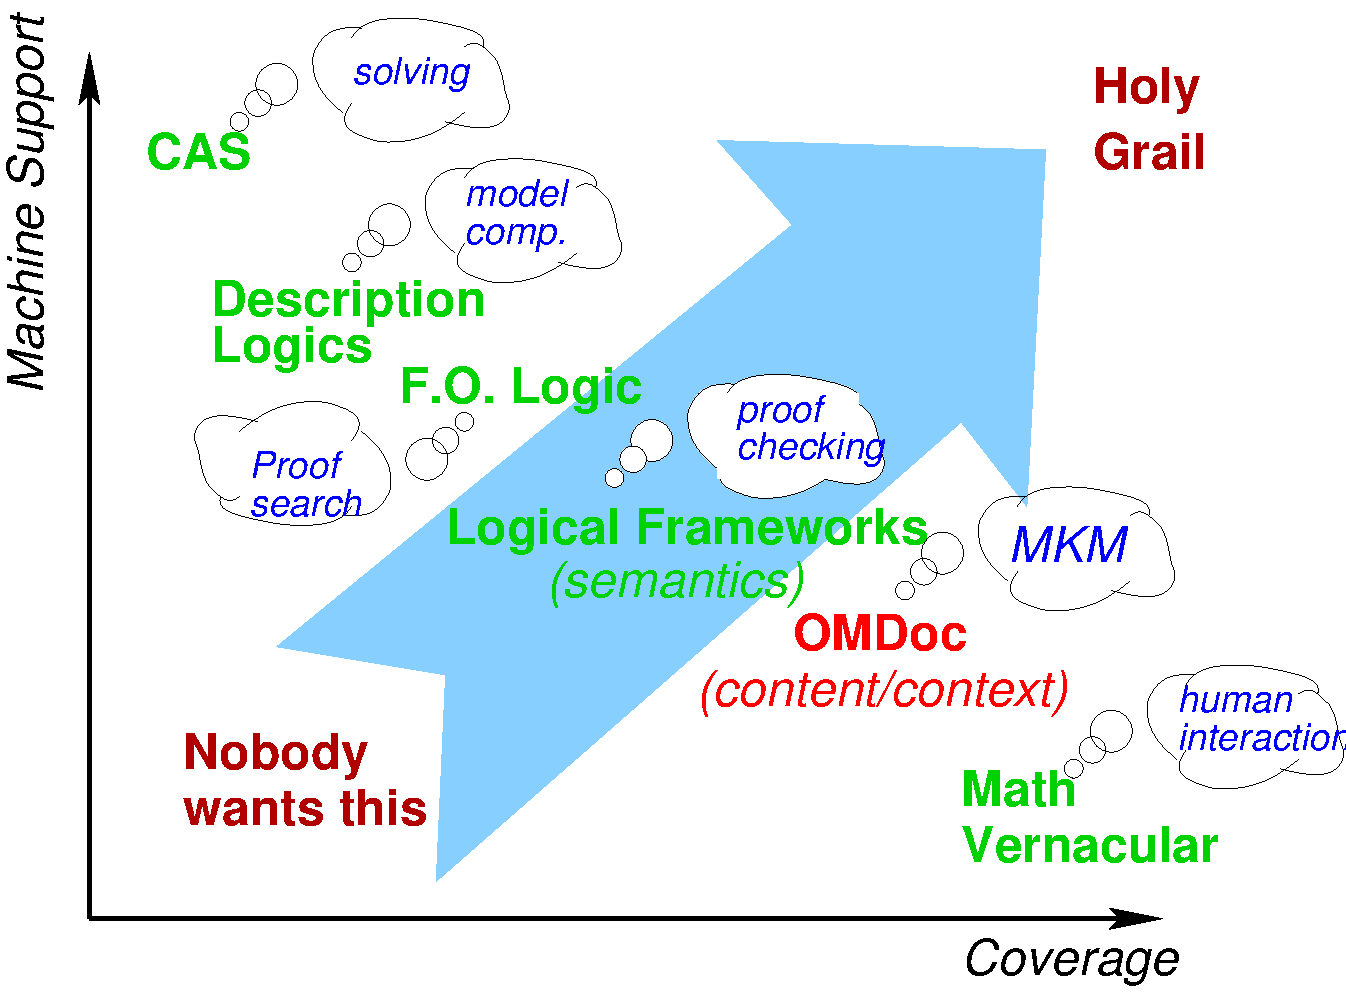
\includegraphics[width=11cm]{figures/support-coverage}
\end{myfig}

On the left hand side we see {\indextoo{CAS}} like {\mathematica}\cite{Wolfram.02} or
{\maple} {\cite{ChaGed:flatim92}} that are relatively restricted in the mathematical
objects --- they can deal with {\indextoo{polynomial}s}, {\indextoo{group
    representation}s}, {\twintoo{differential}{equation}s} only, but in this domain they
can offer sophisticated services like equation solving, factorization, etc.  More to the
right we see systems like {\indextoo{automated theorem prover}s}\index{theorem prover},
whose language --- usually {\twintoo{first-order}{logic}} --- covers much more of
mathematics, but that cannot perform computational services\footnote{Of course in
  principle, the systems could, since computation and theorem proving are inter-reducible,
  but in practice theorem provers get lost in the search spaces induced by computational
  tasks.}  like the CAS do.

In the lower right hand corner, we find languages like
``{\twintoo{mathematical}{vernacular}}'', which is just the everyday mathematical
language. Here coverage is essentially universal: we can use this language to write
international treaties, math books, and love letters; but machine support is minimal,
except for typesetting systems for mathematical formulae like {\TeX}, or keyword search in
the natural language part.

The distribution of the systems clusters around the diagonal stretching from low-coverage,
high-support systems like CAS to wide-coverage, low-support natural language systems. This
suggests that there is a trade-off between coverage and machine support. All of the
representation languages occupy legitimate places in the space of representation
languages, trying to find sweet-spots along this coverage/support trade-off. {\omdoc}
tries to occupy the ``{\twintoo{content}{markup}}'' position. To understand this position
better, let us contrast it to the ``{\twintoo{semantic}{markup}}'' position immediately to
the left of and above it. This is an important distinction, since it marks the border
between formal and {\twintoo{informal}{mathematics}}\twin{formal}{mathematics}.

We define a {\atwindef{semantic}{markup}{format}} (aka {\twindef{formal}{system}}) as a
representation system that has a way of specifying when a formula is a
{\indextoo{consequence}} of another. Many semantic markup formats express the
{\twintoo{consequence}{relation}} by means of a {\twintoo{formal}{calculus}}, which allows
the mechanization of {\twintoo{proof}{checking}} or {\twintoo{proof}{verification}}. It is
a widely held belief in mathematics, that all mathematical knowledge can in principle be
expressed in a {\twintoo{formal}{system}}, and various systems have been proposed and
applied to specific areas of mathematics. The advantage of having a well-defined
consequence relation (and proof-checking) has to be paid for by committing to a particular
logical system.

{\twindef{Content}{markup}} does not commit to a particular consequence relation, and
concentrates on providing services based on the marked up structure of the content and the
context.  Consider for instance the logical formula in {\mylstref{om-comm}}, where the
{\openmath} representation does not specify the full consequence relation (or the
{\twintoo{formal}{system}}) for the formula. It does something less but still useful,
which is what we could call {\twinemph{semantics by}{pointing}}: The symbols used in the
representation are identified by a pointer (the {\indextoo{URI}} jointly specified in the
{\attribute[ns-elt=om]{cd}{OMS}} and {\attribute[ns-elt=om]{name}{OMS}} attributes) to a
defining document (in this case an {\openmath} {\indextoo{content dictionary}}). Note that
URI equality is a sufficient condition for two symbols to be equal, but not a necessary
condition: Two symbols can be semantically equal without pointing to the same document,
e.g.  if the two defining documents are semantically marked up and the definitions are
semantic consequences of each other.

In this sense, content markup offers a more generic markup service (for all formal
systems; we do not have to commit ourselves) at the cost of being less precise (we for
instance miss out on some symbol equalities). Thus, {\twintoo{content}{markup}} is placed
to the lower right of {\twintoo{semantic}{markup}} in {\myfigref{situating}}.  Note
however, that content markup can easily be turned into semantic markup by adding a
consequence relation, e.g. by pointing to defining documents that are marked up
semantically.  Unlike {\openmath} and {\cmathml}, the {\omdoc} format straddles the
content/semantics border by closing the loop and providing a content markup format for
both formulae and the defining documents. In particular, {\emph{an {\omdoc} document is
    semantic if all the documents it references are}}.

As a consequence, {\omdoc} can serve as a {\twintoo{migration}{format}} from formal to
informal mathematics (and thus from representations that for human consumption to such
that can be supported by machines). A document collection can be marked for content and
context structure, making the structures and context references explicit in a first
pass. Note that this pass may involve creating additional documents or identifying
existing documents that serve as targets for the context references so that the document
collection is self-contained.  In a second (and possible semi-automatic) step, we can turn
this self-contained document collection into a formal representation (semantic markup) by
committing on consequence relations and adding the necessary detail to the referenced
documents.
\end{tsection}

\begin{tsection}[id=mathweb]{The Future: An Active Web of (Mathematical) Knowledge}
It is a crucial -- if relatively obvious -- insight that true cooperation of
mathematical services is only feasible if they have access to a joint corpus of
mathematical knowledge. Moreover, having such a corpus would allow to develop
added-value services like
\begin{itemize}
\item Cut and paste on the level of computation (take the output from a web search engine
  and paste it into a computer algebra system),
\item Automatically proof checking published proofs,
\item Math explanation (e.g. specializing a proof to an example that simplifies the proof
  in this special case),
\item Semantic search for mathematical concepts (rather than keywords),
\item Data mining for representation theorems (are there unnoticed groups out there?),
\item Classification: Given a concrete mathematical structure, is there a general theory
  for it?
\end{itemize}
As the online mathematical knowledge is presently only machine-{\emph{readable}}, but not
machine-{\emph{understandable}}, all of these services can currently only be performed by
humans, limiting the accessibility and thus the potential value of the
information. Services like this will transform the now passive and human-centered fragment
of the Internet that deals with mathematical content, into an active (supported by
semantic services) web of mathematical knowledge.

This promise of activating a web of knowledge is not limited to mathematics: the task of
transforming the current presentation-oriented world-wide web into a ``Semantic
Web''~\cite{BernersLee:tsw98} has been identified as one of the main challenges by the
world {\indextoo{W3C}}. With the {\omdoc} format we pursue an alternative vision of a
`Semantic Web' for Mathematics. Like {\twintoo{Tim}{Berners-Lee}}'s vision we aim to make
the Web (here mathematical knowledge) machine-understandable instead of merely
machine-readable. However, instead of a top-down metadata-driven approach, which tries to
approximate the content of documents by linking them to web ontologies (expressed in
terminologic logics), we explore a bottom-up approach and focus on making explicit the
intrinsic structure of the underlying scientific knowledge. A connection of documents to
web ontologies is still possible, but a secondary effect.

The direct applications of {\omdoc} (apart from the general effect towards a Semantic Web)
are not confined to mathematics proper either.  The {\mathml} working group in the W3C has
led the way in many web technologies (presenting mathematics on the web taxes the current
web technology to its limits); the endorsement of the {\mathml} standard by the W3
Committee is an explicit testimony to this. We expect that the effort of creating an
infrastructure for digital mathematical libraries will play a similar role, since
mathematical knowledge is the most rigorous and condensed form of knowledge and will
therefore pinpoint the problems and possibilities of the semantic web.

All modern sciences have a strongly mathematicised core and will benefit. The real market
and application area for the techniques developed in this project lies with high-tech and
engineering corporations that rely on huge formula databases.  Currently, both the content
markup as well as the added-value services alluded to above are very underdeveloped,
limiting the usefulness of vital knowledge. The content-markup aspect needed for mining
this information treasure is exactly what we are developing in {\omdoc}.
\end{tsection}
\end{tchapter}



%%% Local Variables: 
%%% mode: latex
%%% TeX-master: "omdoc"
%%% End: 

% LocalWords:  mobj arith cd nat mathescape eq comm rec om ns elt rpc Bundy th
% LocalWords:  CMP FMP OMA OMV CAS online metadata Andrzej Trybulec Berners
